\documentclass{article}
\usepackage{hyperref}
\usepackage[utf8]{inputenc}
\usepackage[margin=0.2in]{geometry}
\usepackage{amsmath}
\newcommand{\stirlingii}{\genfrac{\{}{\}}{0pt}{}}

\title{Formelblad: Diskret matematik}

\usepackage[usestackEOL]{stackengine}[2013-10-15]
\def\x{\hspace{3ex}}    %BETWEEN TWO 1-DIGIT NUMBERS
\def\y{\hspace{2.45ex}}  %BETWEEN 1 AND 2 DIGIT NUMBERS
\def\z{\hspace{1.9ex}}    %BETWEEN TWO 2-DIGIT NUMBERS
\stackMath

\usepackage{multicol}
\usepackage[table,xcdraw]{xcolor}
\usepackage{tikz}
\usepackage{amsmath}
\usepackage[yyyymmdd,hhmm]{datetime}

\usepackage{algorithm}
\usepackage[ampersand]{easylist}
\usepackage[noend]{algpseudocode}

\usepackage{natbib}
\usepackage{amssymb}
\usepackage{graphicx}
\usepackage{lipsum}% dummy text
\usepackage{mathtools}% http://ctan.org/pkg/mathtools

\begin{document}
\begin{multicols}{2}
\section{Talteori\footnote{Compiled on \today\ at \currenttime \ GMT\\\href{https://github.com/SkruvdragarN/Diskret_matematik_formelblad}{\url{GitHub.com/SkruvdragarN/Diskret_matematik_formelblad.git}}}}
\textbf{Definition:} The function $f$ from $X$ to $Y$ is a \textbf{surjection} if every $y$ in $Y$ is a value $f(x)$ for \textit{at least one} $x$ in $X$. It is a \textbf{injection} if every $y$ in $Y$ is a value $f(x)$ for \textit{at most one} $x$ in $X$. It is a \textbf{bijection} if it is both a surjection and an injection, that is, if every $y$ in $Y$ is a value $f(x)$ for \textit{exacly one} $x$ in $X$.\\
\newline
\textbf{Primtal-test}:
\begin{enumerate}
    \item Om talet $t$ kan primtalsfaktoriseras är det inte ett primtal.
    \item Om talet $t$ inte är ett primtal måste talet ha en primtalsfaktor $p \leq \lfloor \sqrt{t} \rfloor$. Exempel: $p \leq \lfloor \sqrt{1019} \rfloor = 31$ (Testa att dela talet med $[2... 31]$, om inget av talen delar $t$ är $t$ ett primtal).
\end{enumerate}
\newline
\textbf{Definition:} If $gcd(a,b) = 1$ then \textbf{coprime}.\\
\newline
\textbf{Theorem 6.2.1}
Let $m$ be a natural number. Then the following statement is true for every natural number $n$: if there is an injection from $\mathbb{Z}_n$ to $\mathbb{Z}_m$, then $n\leq m$. ($\implies$ the \textbf{pigeonhole principle/brevlådeprincipen})\\
\newline
A \textbf{relation} $R$ on a set $X$ is a set of ordered pairs of members of $X$. \textit{R} is \textbf{reflexive} if $xRx$ for every $x \in X$. \textit{R} is \textbf{symmetric} if, whenever we have $xRy$, we also have $yRx$. \textit{R} is \textbf{transitive} if, whenever we have both $xRy$ and $yRz$, we also have $xRz$. $R$ is a \textbf{equivalence relation} if its \textbf{reflexive}, \textbf{symmetric} and \textbf{transitive}.\\
\newline
En \textbf{multiplikativ invers} till ett tal $A$ är det tal $B$ som vid multiplikation ger $1$, $AB=1$. Den multiplikativa inversen till talet 2 är 0,5, ty $2*0,5=1$. Under congruence, t.ex. $\mathbb{Z}_{113}$ se \ref{congur}.


\subsection{Byta talbas}
\begin{multicols}{2}
Exempel: $(109)_{10} = (1101101)_2$
$$109 = 2 \times 54 + 1$$
$$54 = 2 \times 27 + 0$$
$$27 = 2 \times 13 + 1$$
$$13 = 2 \times 6 + 1$$
$$6 = 2 \times 3 + 0$$
$$3 = 2 \times 1 + 1$$
$$1 = 2 \times \textbf{0} + 1$$
\end{multicols}


\subsection{Hitta $gcd(x,y)$ (Euclidean algorithm)}\label{euclid}
$gcd(2406,654)$
$$2406 = 654 \times 3 + 444 \implies gcd(2406,654) = gcd(654,444)$$
$$654 = 444 \times 1 + 210 \implies gcd(2406,654) = gcd(444,210)$$
$$444 = 210 \times 2 + 24 \implies gcd(2406,654) = gcd(210,24)$$
$$210 = 24 \times 8 + 18 \implies gcd(2406,654) = gcd(24,18)$$
$$24 = 18 \times 1 + 6 \implies gcd(2406,654) = gcd(16,6)$$
$$18 = 6 \times 3 \implies gcd(2406,654) = gcd(6,0) = \textbf{6}$$
\newline
Tillämpning: Antal 13-liter-hinkar $x$ och 31-liter-hinkar $y$ för att få 3 liter, $13x+31y=3$. Ges av att lösa $13x+31y=1$ utifrån resultatet från euklides och därefter multiplicera med 3. Euklides:
$$31=13*2+5 \rightarrow 13=5*2+3 \rightarrow 5=3*2+2 \rightarrow 3=1*2+1$$
Algebra utifrån euklides-resultat:\\
$1=3*2=3-(5-3)=(-1)*5+2*3=(-1)*5+2*(13-2*5)=$\\
$=(-5)*5+2*13=(-5)(31-2*13)+2*13=$\\
$(-5)*31+12*13=1$\\ 
Multiplicera med 3 $\rightarrow 13(3*13)+31(-5*3)=3$\\
$x=36 \quad y=-16$

\section{Enumerationsproblem}
$$\sum_{k=1}^{n-1} k = \frac{n(n-1)}{2}$$

\subsection{Kombinatorik}
\fbox{\begin{minipage}{28em}
"Ur en mängd med storlek $n$ välj ut $r$ stycken."
\subsubsection{Ordered | Without repetition}
$$\frac{n!}{(n-r)!} = n(n-1)...(n-r+1)$$
Pallplaceringar (tävling). Antalet injektioner mellan mängder $f: N_r \rightarrow N_n$ med storlek $r$ och $n$.
\subsubsection{Unordered | Without repetition}
$$\binom{n}{r}$$
Hur många olika händer kan man få givna i poker?
\subsubsection{Ordered | With repetition}
$$n^r$$
Pinkoder. Binära tal med 13 siffror? ($2^{12}$ inte börja med 0)
\subsubsection{Unordered | With repetition}
$$\binom{n-1+r}{r}$$
Antal sätt man kan slå 4 tärningar? Lösningar till $x + y + z + w = 45$ där $x,y,z,w \in \mathbb{N}$ ger $n=4 \ r=45$, dvs $\binom{4-1+45}{45}$.

\end{minipage}}

\subsection{Euler's phi-funktion $\phi(n)$}

$\phi(n)$ is the number of non-negative integers less than $n$ that are relatively prime (coprime) to $n$.

$$\phi(n)=\phi(p^{\varepsilon_1}_1*p^{\varepsilon_2}_2*...*p^{\varepsilon_k}_k)$$
där $p^{\varepsilon_n}_n$ är primtal i primtalsfaktoriseringen av $n$.

$$\phi(p) = p-1 \quad \quad \phi(p^\varepsilon) = p^\varepsilon-p^{\varepsilon-1}$$
Där $p$ är ett primtal.

$$\phi(a*b) = \phi(a)*\phi(b) \quad om \ gcd(a,b)=1$$

\subsection{Permutations}

Cyklisk notation: $\alpha = (124)(35)$ och $\beta = (13)(25)(4)$ ger:\\
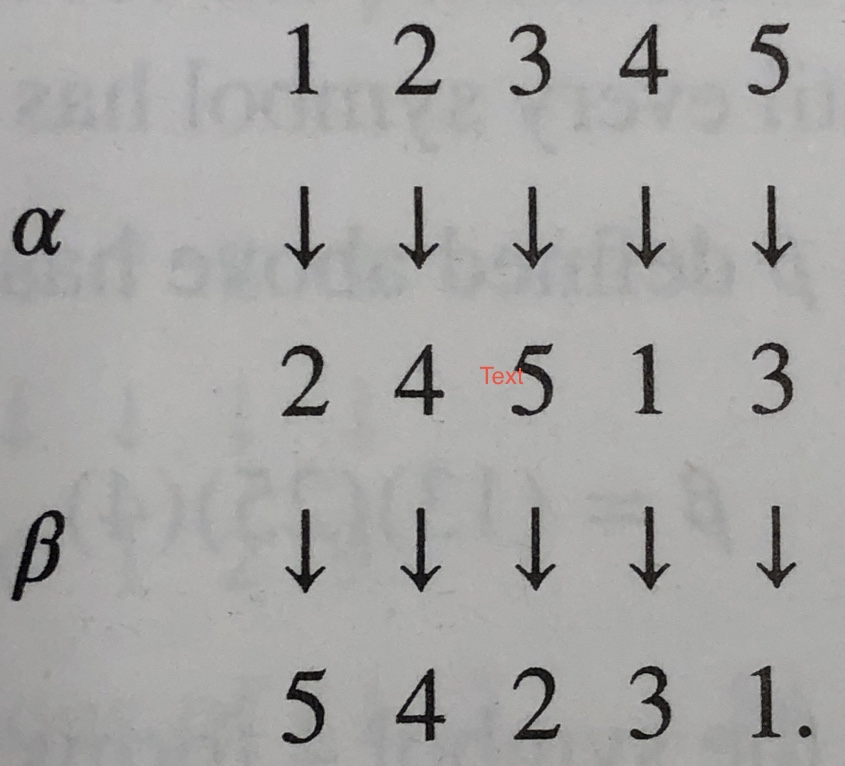
\includegraphics[width=0.12\textwidth]{images/partition}\\ Dvs $\beta \alpha = (15)(243)$. Först $\alpha$ sedan $\beta$. 
För att återfå samma permutation kan du blanda $k$ gånger. Där $k$ är den minsta gemensamma nämnare av cyklernas storlek. Minsta gemensamma nämnare till 2 och 8 är 8. Invers: $(\beta \alpha)^{-1} = (51)(342)$

\subsection{Binomial numbers}
\textbf{Theorem 11.1.1 + 11.1.2}
$$\binom{n}{r} = \binom{n-1}{r-1} + \binom{n-1}{r} = \frac{n!}{r!(n-r)!}$$
\newline
\textbf{Pascals triangel}
\hspace{10pt}

\Longstack[l]{
n=0\\
n=1\\
n=2\\
n=3\\
n=4\qquad\ \\
}
\Longstack{
1\\
1\x 1\\
1\x 2\x 1\\
1\x 3\x 3\x 1\\
1\x 4\x 6\x 4\x 1\\
}

\subsection{Binomial theorem}
\textbf{Theorem 11.3}
$$(a+b)^n = \binom{n}{0}a^n + \binom{n}{1}a^{n-1}b + \binom{n}{2}a^{n-2}b^2 + ... + \binom{n}{n}b^n$$
$$(a+b)^n = \sum_{k=0}^{n} \binom{n}{k}(a^{n-k}*b^k)$$

\subsection{The sieve principle (Sållningsprincipen)}
\textbf{Theorem 11.4}\\
If $A_1,A_2,...,A_n$ are finite sets then
$$|A_1 \cup A_2 \cup ... \cup A_n| = a_1 - a_2 + a_3 -...+(-1)^{n-1}*a_n$$
where $a_i$ is the sum of the cardinalities of the intersections of the sets taken $i$ at a time $(1 \leq i \leq n)$.\\
\newline
Exempel: 
\\Heltal $1 \leq n \leq 1000$ där $n$ är delbar med minst en av $3,5,7$:\\
$|A_3 \cup A_5 \cup A_7|=$\\
$|A_3|+|A_5|+|A_7| - (|A_3 \cap A_5|+|A_3 \cap A_7|+|A_5 \cap A_7|) + (|A_3 \cap A_5 \cap A_7|)$\\
$\lfloor \frac{1000}{3} \rfloor + \lfloor \frac{1000}{5} \rfloor + \lfloor \frac{1000}{7} \rfloor - (\lfloor \frac{1000}{3*5} \rfloor + \lfloor \frac{1000}{3*7} \rfloor + \lfloor \frac{1000}{5*7} \rfloor) + \lfloor \frac{1000}{3*5*7} \rfloor = 544$

\subsection{Partitions}
\textbf{Definition:} A \textbf{partition} of a set $X$ is a family $\{X_i | i \in I\}$ of non-empty subsets of $X$ such that 
\begin{itemize}
    \item $X$ is the union of the sets $X_i \ (i \in I)$,
    \item each pair $X_i,X_j \ (i \ne j)$ is disjoint
\end{itemize}
The subsets $X_i$ are called the \textbf{parts} of the partition.\\
\newline
\textbf{Theorem 12.1}\\
Let $S(n,k)$ denote the number of partitions of an $n$-set $X$ into $k$ parts, where $1 \leq k \leq n$. Then

$$S(n,1)=1, \quad S(n,n)=1,$$
$$S(n,k) = S(n-1,k-1) + kS(n-1,k) \quad (2 \leq k \leq n-1)$$
\newline
The number $S(n,k)$ are sometimes called \textbf{Stirling numbers} (of the second kind). Can be tabulated as below.

\hspace{10pt}

\Longstack[l]{
n=1\\
n=2\\
n=3\\
n=4\\
n=5\\
n=6\\
n=7\qquad\ \\
}
\Longstack{
1\\
1\x 1\\
1\x 3\x 1\\
1\x 7\x 6\x 1\\
1\x 15\x 25\x 10\x 1\\
1\x 31\y 90\z 65\y 15\x 1\\
1\x 63\y 301\z 350\z 140\y 21\x 1\\
}

\subsection{Distributions and multinomial numbers}\label{multiNom}
\textbf{Theorem 12.3.2}\\
Given any positive integers $n, n_1,...,n_k$ satisfying $n_1+n_2+...+n_k=n$, we have
$$\binom{n}{n_1,n_2,...,n_k} = \frac{n!}{n_1!n_2!...n_k!}$$ Kallas ett \textit{multinomial number}. Exempel: How many 11-letter words can be made from the letters of the word ABRACADABRA? Ger antal A $n_1=5$, antal B $n_2=2$, antal R $n_3=2$ etc.\\
\newline
\textbf{Theorem 12.3.3}\\
For any positive integers $n$ and $k$
$$(x_1 + x_2 +...+ x_k)^n = \sum \binom{n}{n_1,n_2,...,n_k} = x_1^{n_1}x_2^{n_2}...x_k^{n_k}$$
Notera att $\binom{n}{n_1,n_2,...,n_k}$ är det ett \textit{multinomial number}, se ovan.

\subsection{Concurrence $x_1 \equiv x_2 \ (mod \ m)$} \label{congur}
\textbf{Definition:} Let $x_1$ and $x_2$ be integers, and $m$ a positive integer. We say that $x_1$ is \textbf{congurent} to $x_2$ \textbf{modulo} $m$, and write $x_1 \equiv x_2 \ (mod \ m)$ whenever $x_1-x_2$ is divisible by $m$.\\
\newline
\textbf{Definition:} The set of \textbf{integers modulo m}, written as $\mathbb{Z}_m$, is the set of distinct equivalence classes under the relation of congruence modulo $m$ in $\mathbb{Z}$. Exempel: $\mathbb{Z}_3 = \{X_0 \cup X_1 \cup X_2\}$, where
$X_0 = [0]_3 = \{...,-3,0,3,6,...\} \quad X_1 = [1]_3 = \{...,-2,1,4,7,...\} \quad X_2 = [2]_3 = \{...,-1,2,5,8,...\}$ \quad $7+5=0 \ (i \ \mathbb{Z}_3) \ \iff \ [7]_3 \oplus [5]_3 = [0]_3$\\
\newline
Talen i $X_P = [P]_3$ har alla rest $P$ vid division med 3.\\
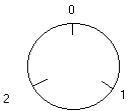
\includegraphics[width=0.095\textwidth]{images/mod}

\includegraphics[width=0.3\textwidth]{images/this_is_fine}\\
\textbf{Theorem 13.3.1}\\
The element $r$ in $\mathbb{Z}_m$ is invertible if and only if $r$ and $m$ are coprime in $\mathbb{Z}$. In particular, when $p$ is a prime every element of $\mathbb{Z}_p$ except 0 is invertible.\\
\newline
\textbf{Theorem 13.3.2}\\
If $y$ is invertible in $\mathbb{Z}_m$ then $y^{\phi(m)}=1 \ in \ \mathbb{Z}_m$\\
\newline
\textbf{Multiplikativ invers} i t.ex. $\mathbb{Z}_{113}$. Använd euclides (\ref{euclid}) och algebra-jonglera uttrycket till $32x + 113k = 1$ ($113k=0$ och $32*53=1$ i $\mathbb{Z}_{113}$).

\section{Grafteori och algoritmer}
\textbf{Binära metoden för exponentiering:}\\
Beräkna $2^{50}$ med 7 multiplikationer istället för 49. Skriv exponenten som summa av 2-potenser $50=32+16+2=2^5+2^4+2^1$. Vi beräknar potenserna $2^1,2^2,2^4,2^8,2^{16},2^{32}$ genom att kvadrera föregående potens i listan (5 multiplikationer). Vi kan därefter beräkna $2^{50}=2^{32+16+2}=2^{32}*2^{16}*2^2$ (2 multiplikationer till).\\
\newline
\textbf{Definition:} A \textbf{graph} $G$ consists of a finite set $V$, whose members are called \textbf{vertices}, and a set $E$ of 2-subsets of $V$, whose members are called \textbf{edges}. We usually write $G = (V,E)$ and say that $V$ is the \textbf{vertex set} and $E$ is the \textbf{edge set}.\\
\newline
\textbf{Definition:} Two graphs $G_1$ and $G_2$ are said to b \textbf{isomorphic} when there is a bijection $a$ from the vertex set of $G_1$ to the vertex set of $G_2$ such that $\{a(x),a(y)\}$ is an edge of $G_2$ if and only if $\{x,y\}$ is an edge of $G_1$. The bijection $a$ is said to be an \textbf{isomorphism}.\\
\newline
\textbf{Definition:} The \textbf{degree} of a vertex $v$ is a graph $G = (V,E)$ is the number of edges of $G$ which contains $v$. Notation: $\delta(v)$.\\ 
\newline
\textbf{Theorem 15.3}\\
The sum of the values of degree $\delta(v)$, taken over all the vertices $v$ of a graph $G = (V,E)$, is equal to twice the number of edges: 
$$\sum_{v \in V}^{} \delta(v) = 2|E|$$
\textbf{Definition:} A \textbf{walk} in a graph $G$ is a sequence of vertices $v_1, v_2,...,v_k$, such that $v_i$ and $v_{i+1}$ are adjacent $(1 \leq i \leq k-1)$. If all its vertices are distinct, a walk is called a \textbf{path}.\\
\newline
\textbf{Definition:} We say that a graph $T$ is a \textbf{tree} if $T$ is connected and there are no cycles in $T$.\\ 
\newline
Ett \textbf{rotat träd} är träd där man valt ut en nod i trädet, och kallar den för en rot, som utgör basen för trädet. Två rotade träd anser lika endast om det finns en isomorfi från den ena till den andra som avbildar roten från den första till roten av den andra. En \textbf{komplett graf} är en graf där varje par av distinkta hörn har en kant mellan sig. 

\subsection{Vertex colouring}
\textbf{Definition:} A \textbf{vertex colouring} of a graph $G = (V,E)$ is a function $c: V \rightarrow \mathbb{N}$ with the property that $$c(x) \neq c(y) \quad whenever \quad \{x,y\} \in E$$
\newline
\textbf{Definition:} The \textbf{chromatic number} (\textbf{hörnkromatiska talet}) of $G$, written $\chi(G)$, is defined to be the least integer $k$ for which there is vertex colouring $c$ which is a function from $V$ to $\mathbb{N}_k$, and $k$ is the least integer with this property.\\

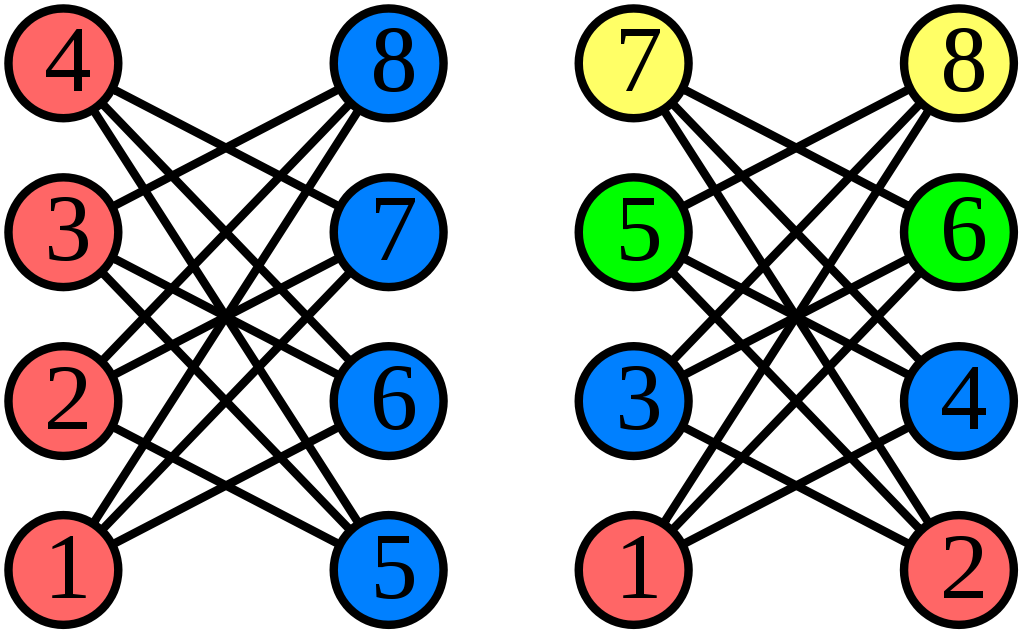
\includegraphics[width=0.15\textwidth]{images/greedy}

\includegraphics[width=0.22\textwidth]{images/knug} 

\subsection{Spanning trees}
Suppose that $G=(V,E)$ is a connected graph, and $T$ is a subset of $E$ such that: \textbf{1.} Every vertex of $G$ belongs to an edge in $T$; \textbf{2.} the edges in $T$ form a tree. In this case, we say that $T$ is a \textbf{spanning tree} for $G$.

\subsection{Sortering}
\subsubsection{Heap sort}
Sorterar listan $4,8,7,1,9,3,2,5,6$. Först fylls noderna i ett binärt träd med elementen i listan.
\begin{multicols}{2}
    \begin{enumerate}
        \item Först fylls noderna i ett binärt träd med elementen i listan.\\
        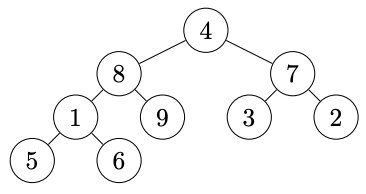
\includegraphics[width=0.2\textwidth]{images/heap1}
        \item Nu ska trädet omvandlas till en heap genom att byta plats på element så att alla fäder innehåller ett lägre värde än sina söner. Vi börjar med delträdet till vänster $(1,5,6)$ och sedan delträdet till höger $(2,3,7)$.\\
        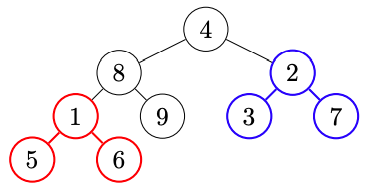
\includegraphics[width=0.2\textwidth]{images/heap2}
        \item Vi fortsätter sedan med det vänstra delträdet $(1,5,9,8,6)$ nedan och byter plats på 8 och 1 följt av 8 och 5.\\
        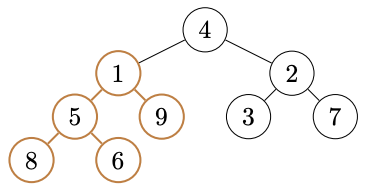
\includegraphics[width=0.2\textwidth]{images/heap3}
        \item Avslutningsvis behandlas hela trädet med bytet mellan 4 och 1.\\
        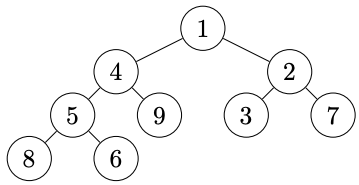
\includegraphics[width=0.2\textwidth]{images/heap4}
        \item Trädet är nu en heap och det minsta elementet finns i roten. Vi tar bort detta element och ersätter det men det element som ligger längst ner till höger, d.v.s. elementet 6. Vi uppdaterar därefter trädet genom att byta plats på 6 och 2 följt av 6 och 3.\\
        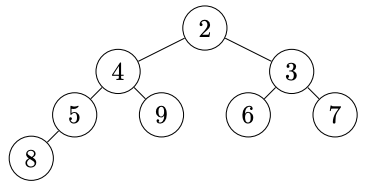
\includegraphics[width=0.2\textwidth]{images/heap5}
    \end{enumerate}
    Antal jämförelser: $O(n*log(n))$. Antal byten: $O(n*log(n))$.
\end{multicols}

\subsubsection{Bubble sort}
Sortering av listan $X = \{x_1,x_2,...,x_n\}$ ger:\\
$for \ j:=1 \ to \ n-1 \ do$\\
$\quad for \ i:=1 \ to \ n-j \ do$\\
$\quad \quad if \ x_i \ > \ x_{i+1} \ then \ switch \ x_i \ and \ x_{i+1}$\\
\newline
Jämförelser (efter $j$te genomgången): $n-j$.\\
Antal jämförelser: $O(n^2)$. Antal byten: $O(n^2)$. 

\subsubsection{Insertion sort}
The basic idea of insertion sorting is to begin with the list $L=(x_1)$ and insert $x_i$ in its correct place in the list for $i =2,3,...,n$. For example, if $x_1,x_2,...,x_8$ are the integers $47,73,21,45,28,69,19,23$, the list is built up as shown below:\\
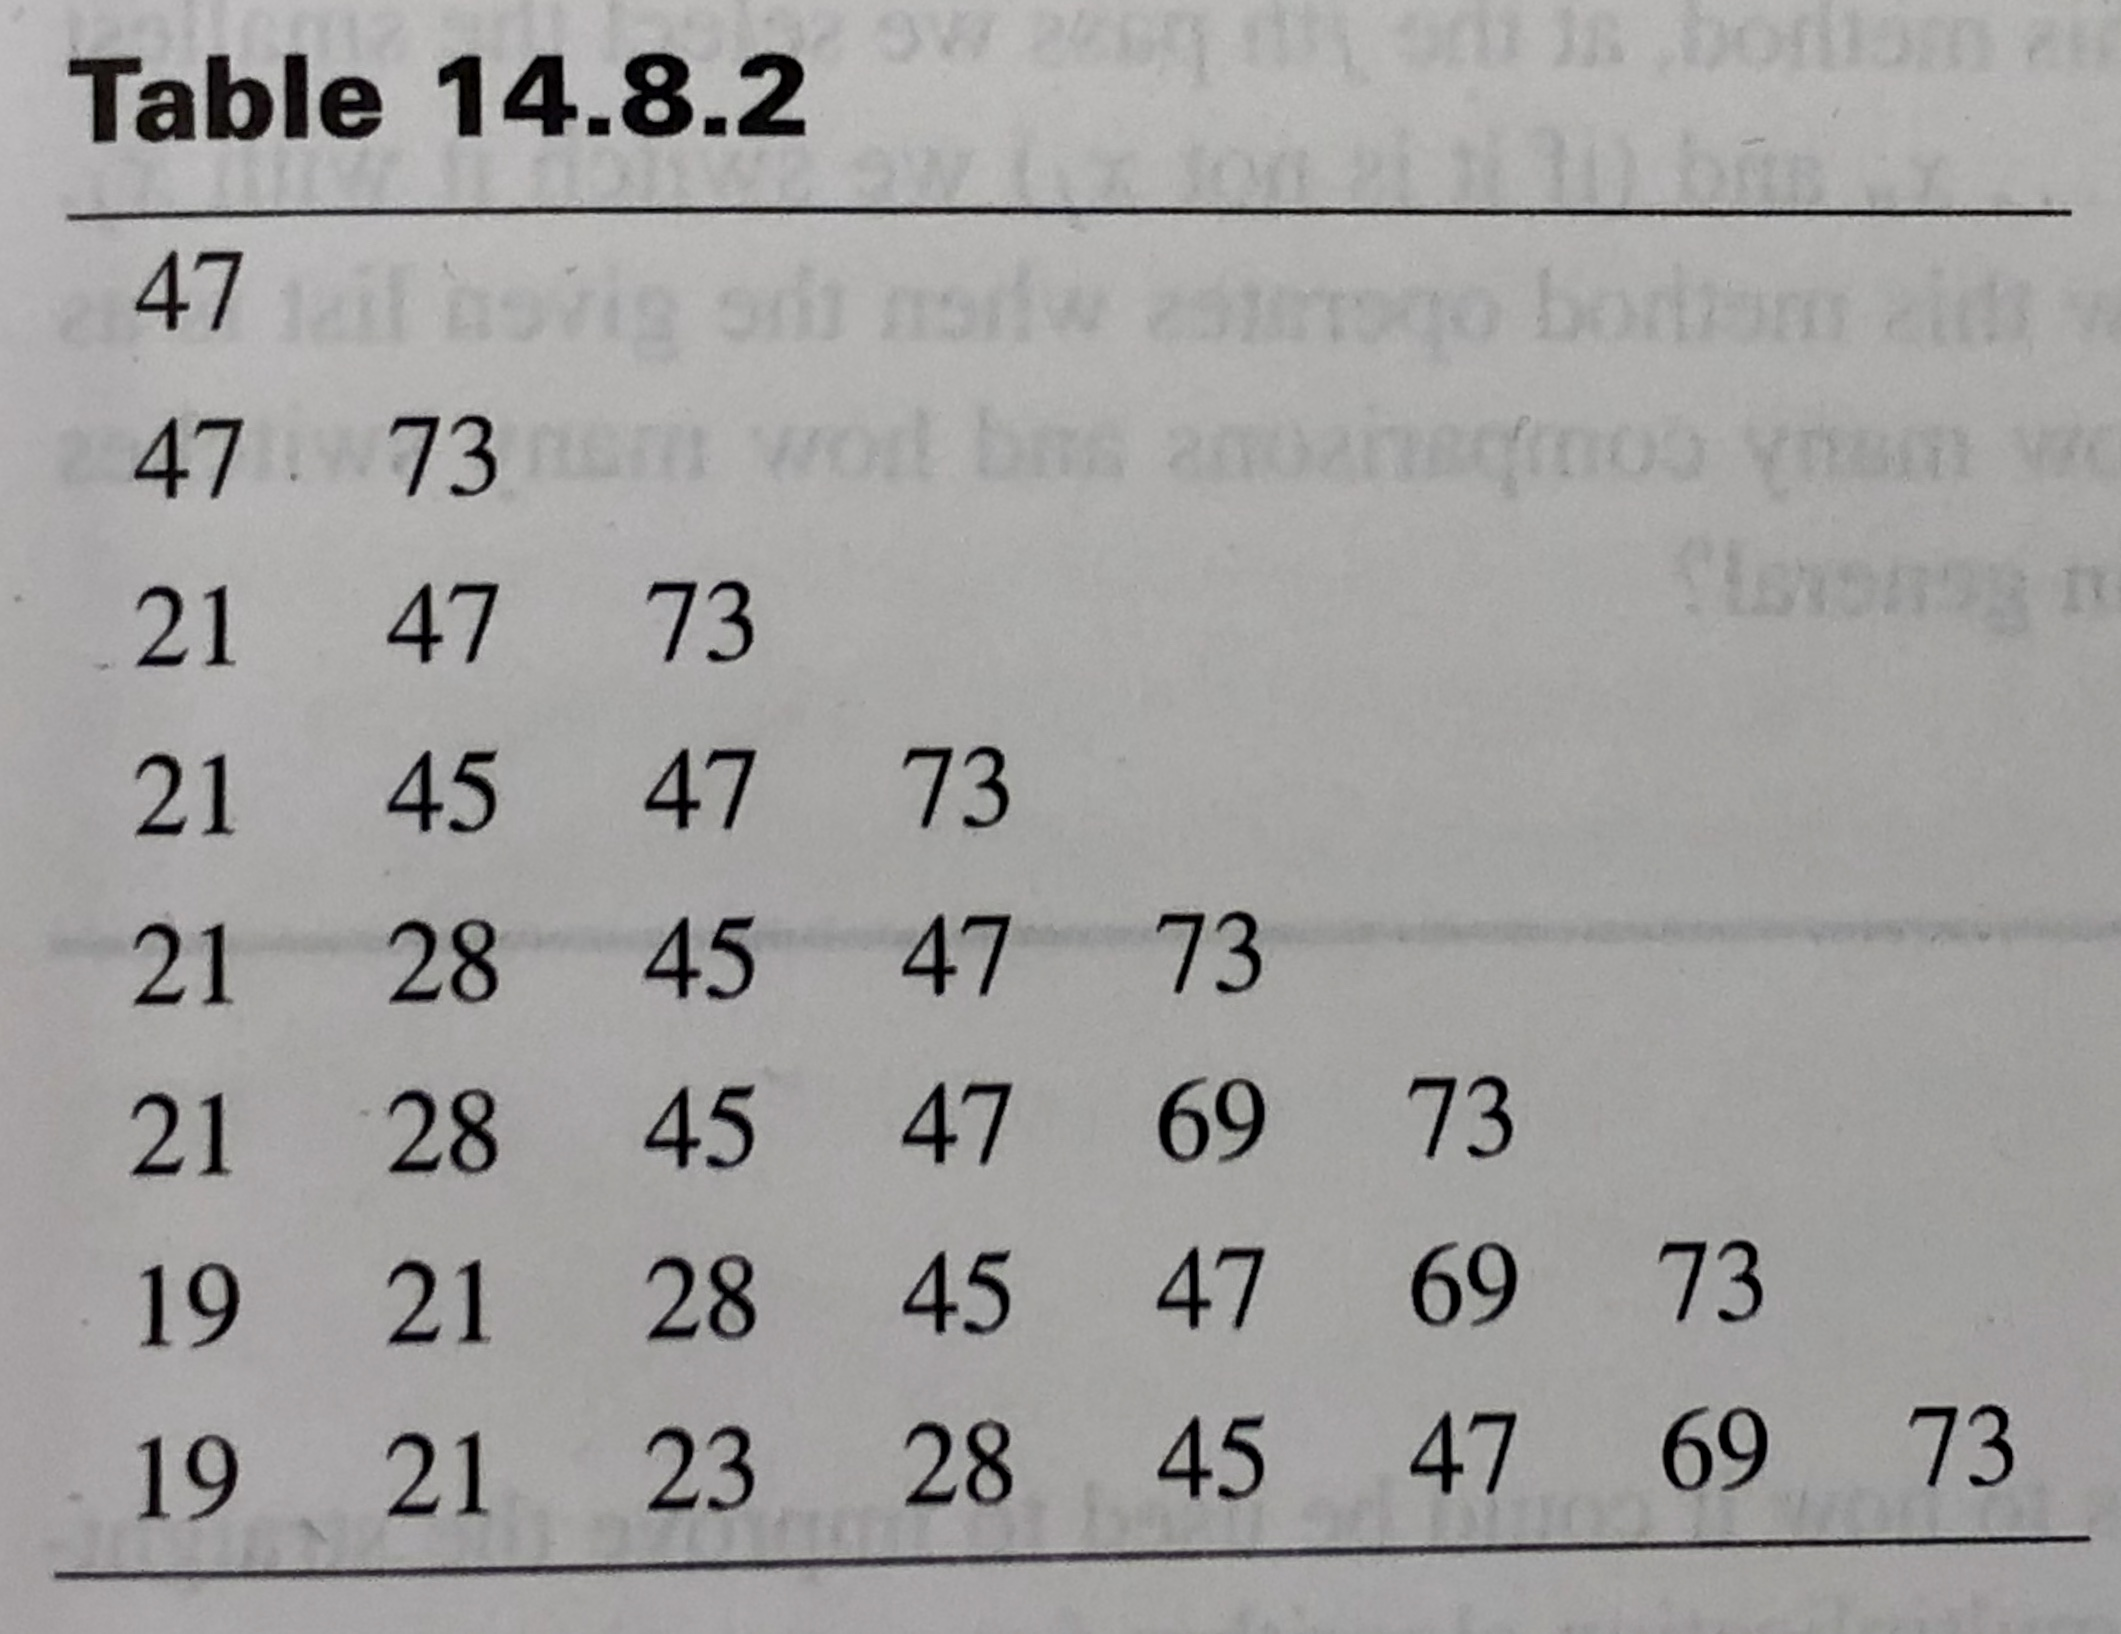
\includegraphics[width=0.21\textwidth]{images/insertion}\\
Antal jämförelser: $O(n*log(n))$. Antal byten: $O(n*log(n))$. Om man använder \textit{bisection} metoden, dvs veta vilken halva av listan som $x$ ska placeras i.

\subsection{Greedy vertex colouring algorithm}
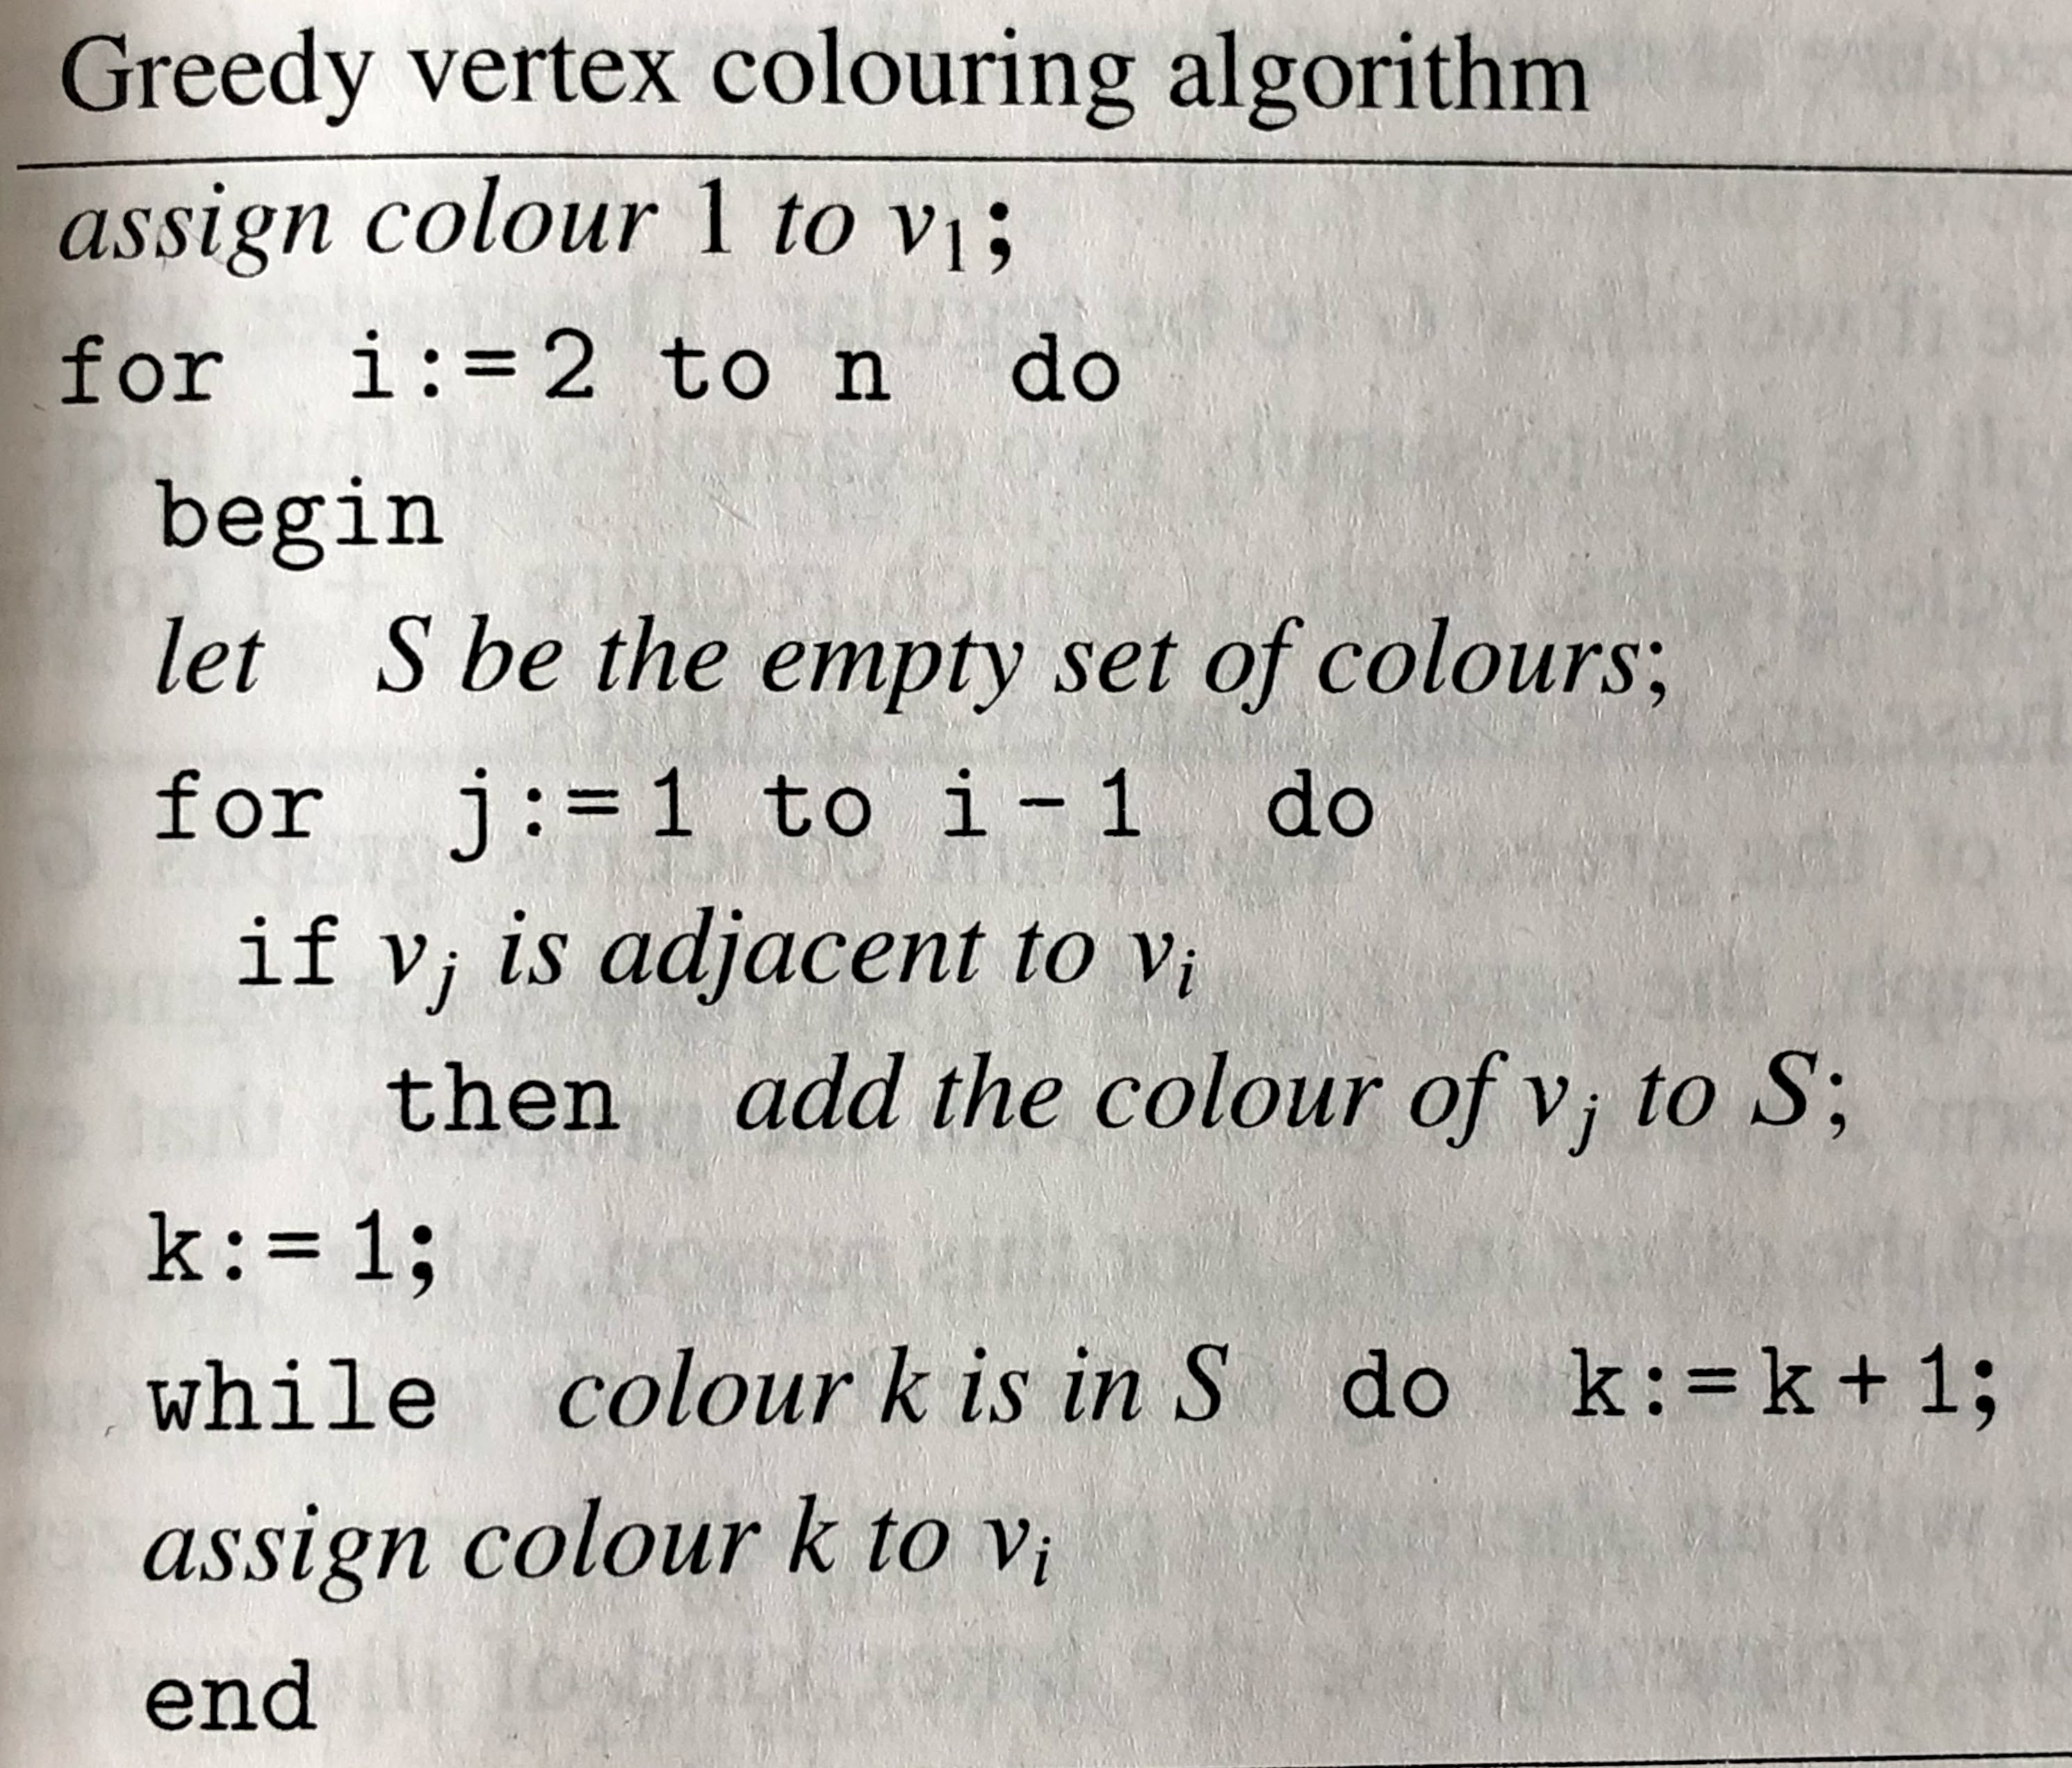
\includegraphics[width=0.23\textwidth]{images/color_alg}\\
Färgningen av kanter får ske i godtycklig ordning.

\subsection{Minimum spanning tree problem (MST)}
At each stage we add the \textit{cheapest} edge joining a new vertex to the partial tree (If several edges with the same weight are available we can select any of them).

\subsection{Depth-first search (DFS)}
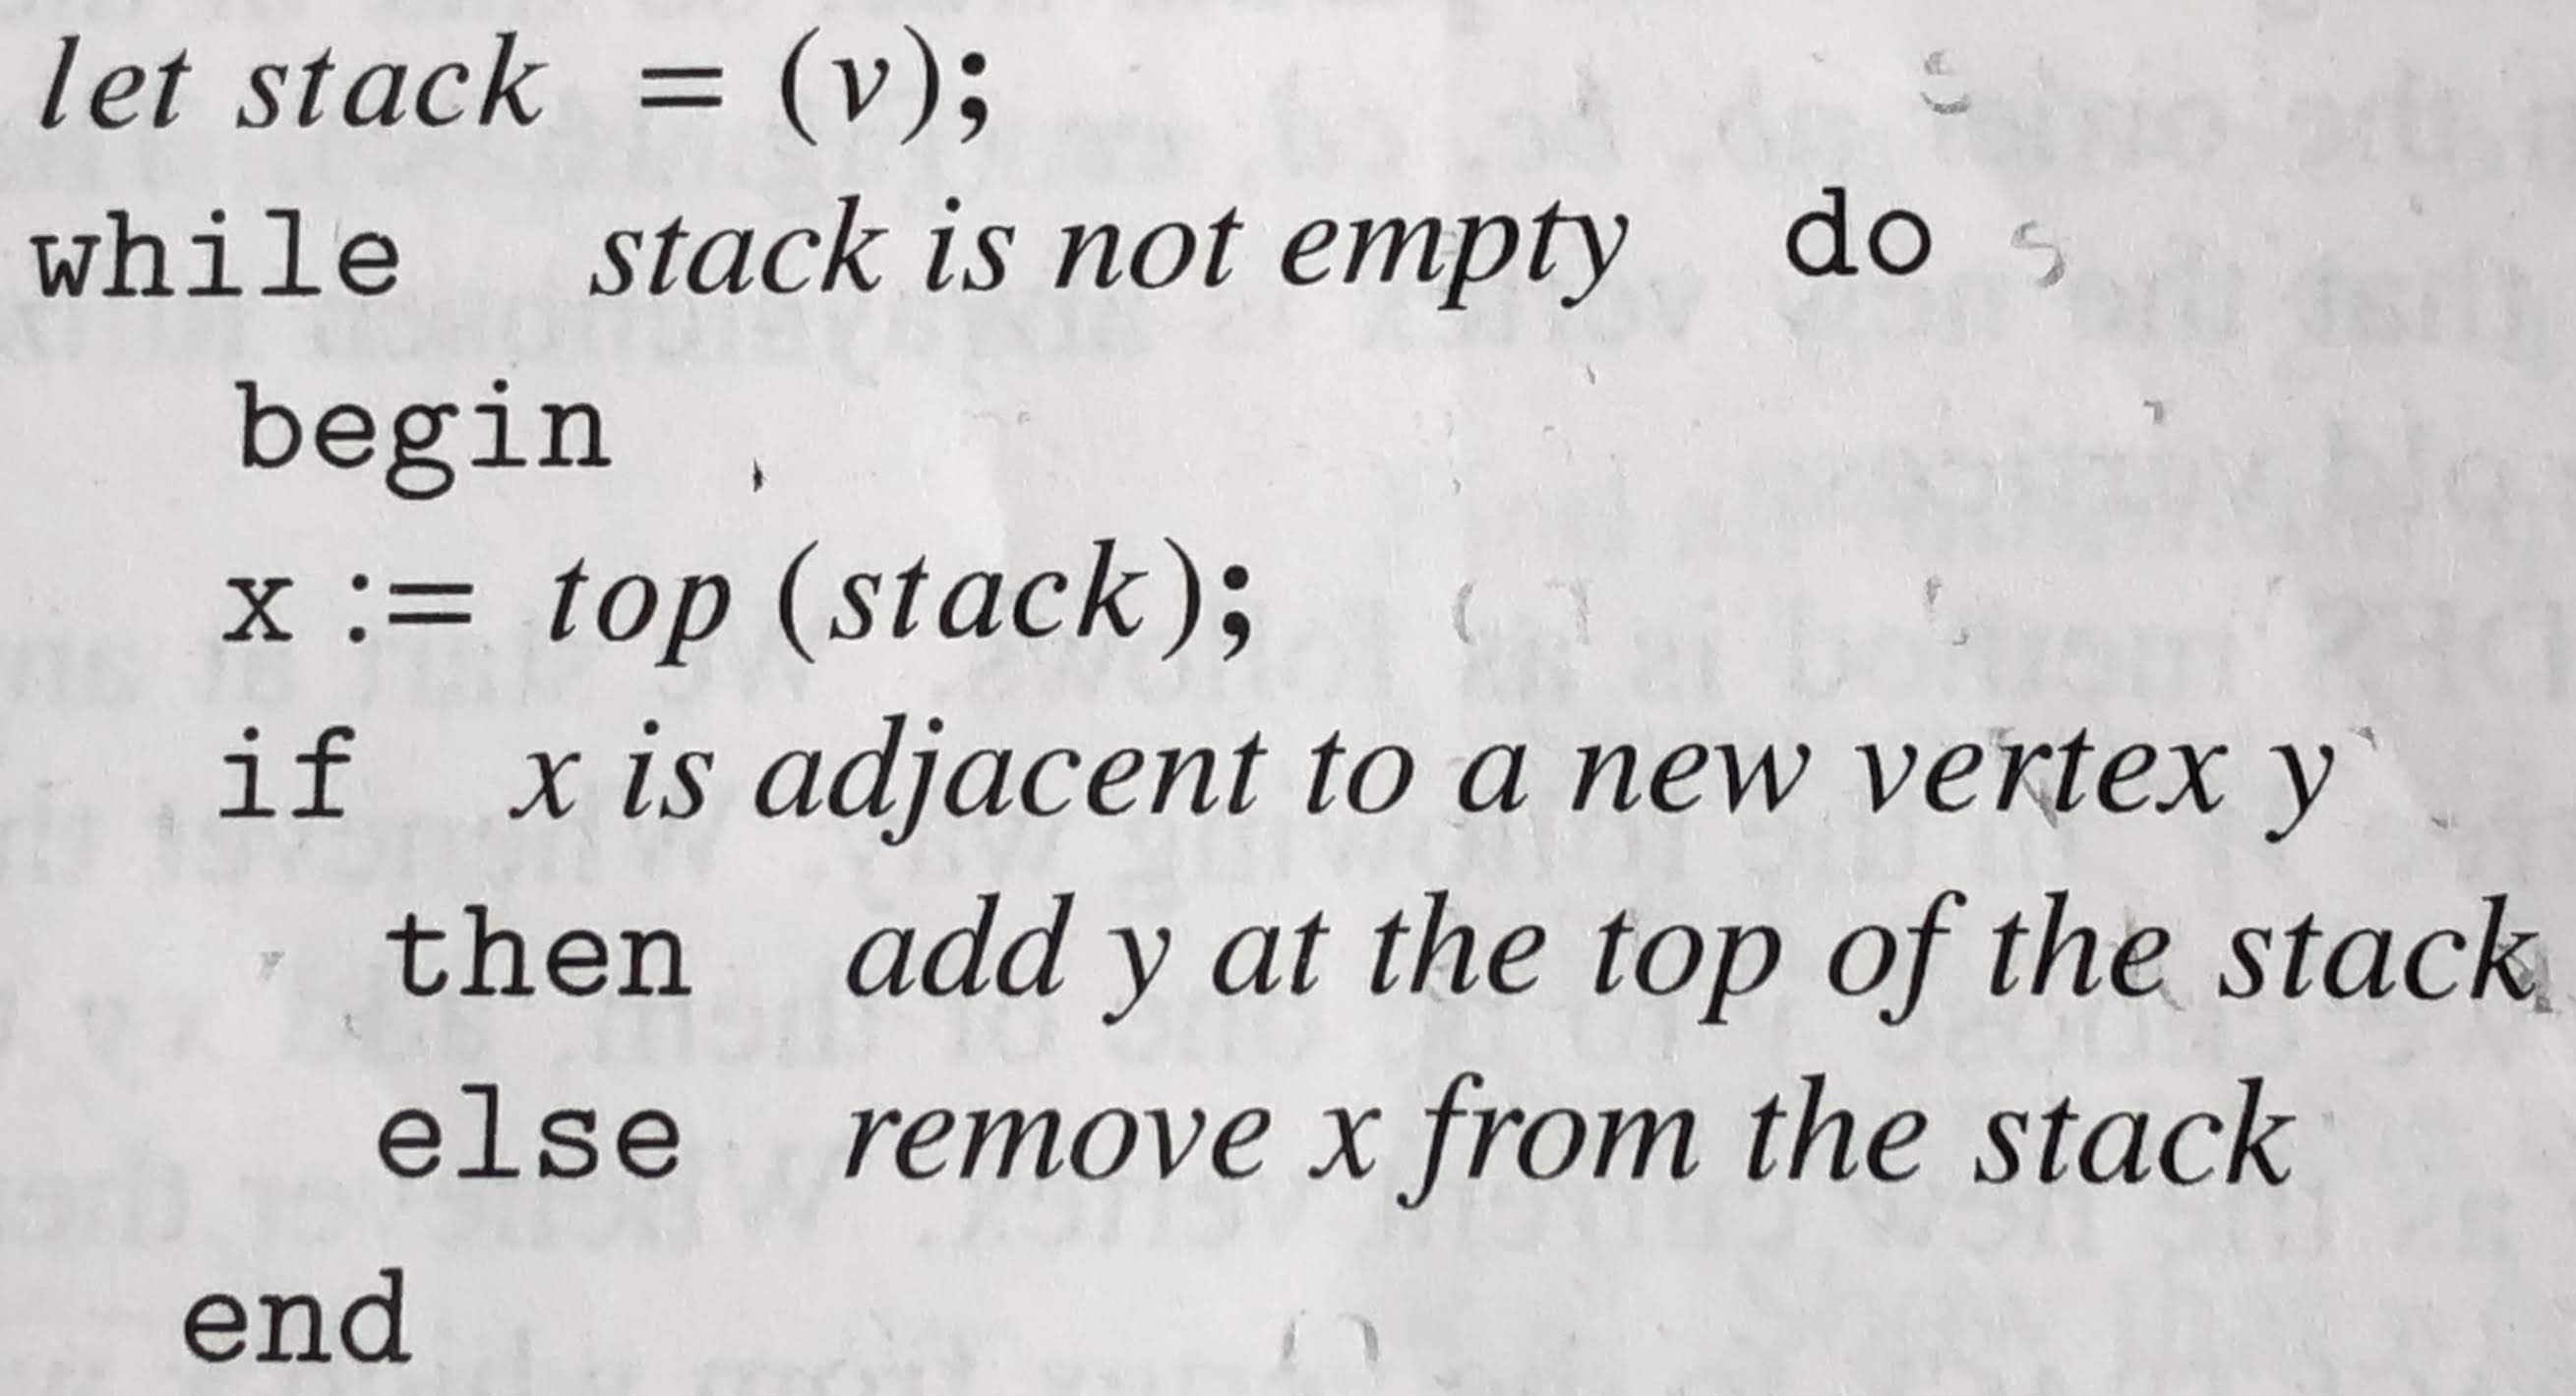
\includegraphics[width=0.25\textwidth]{images/DFS_alg}
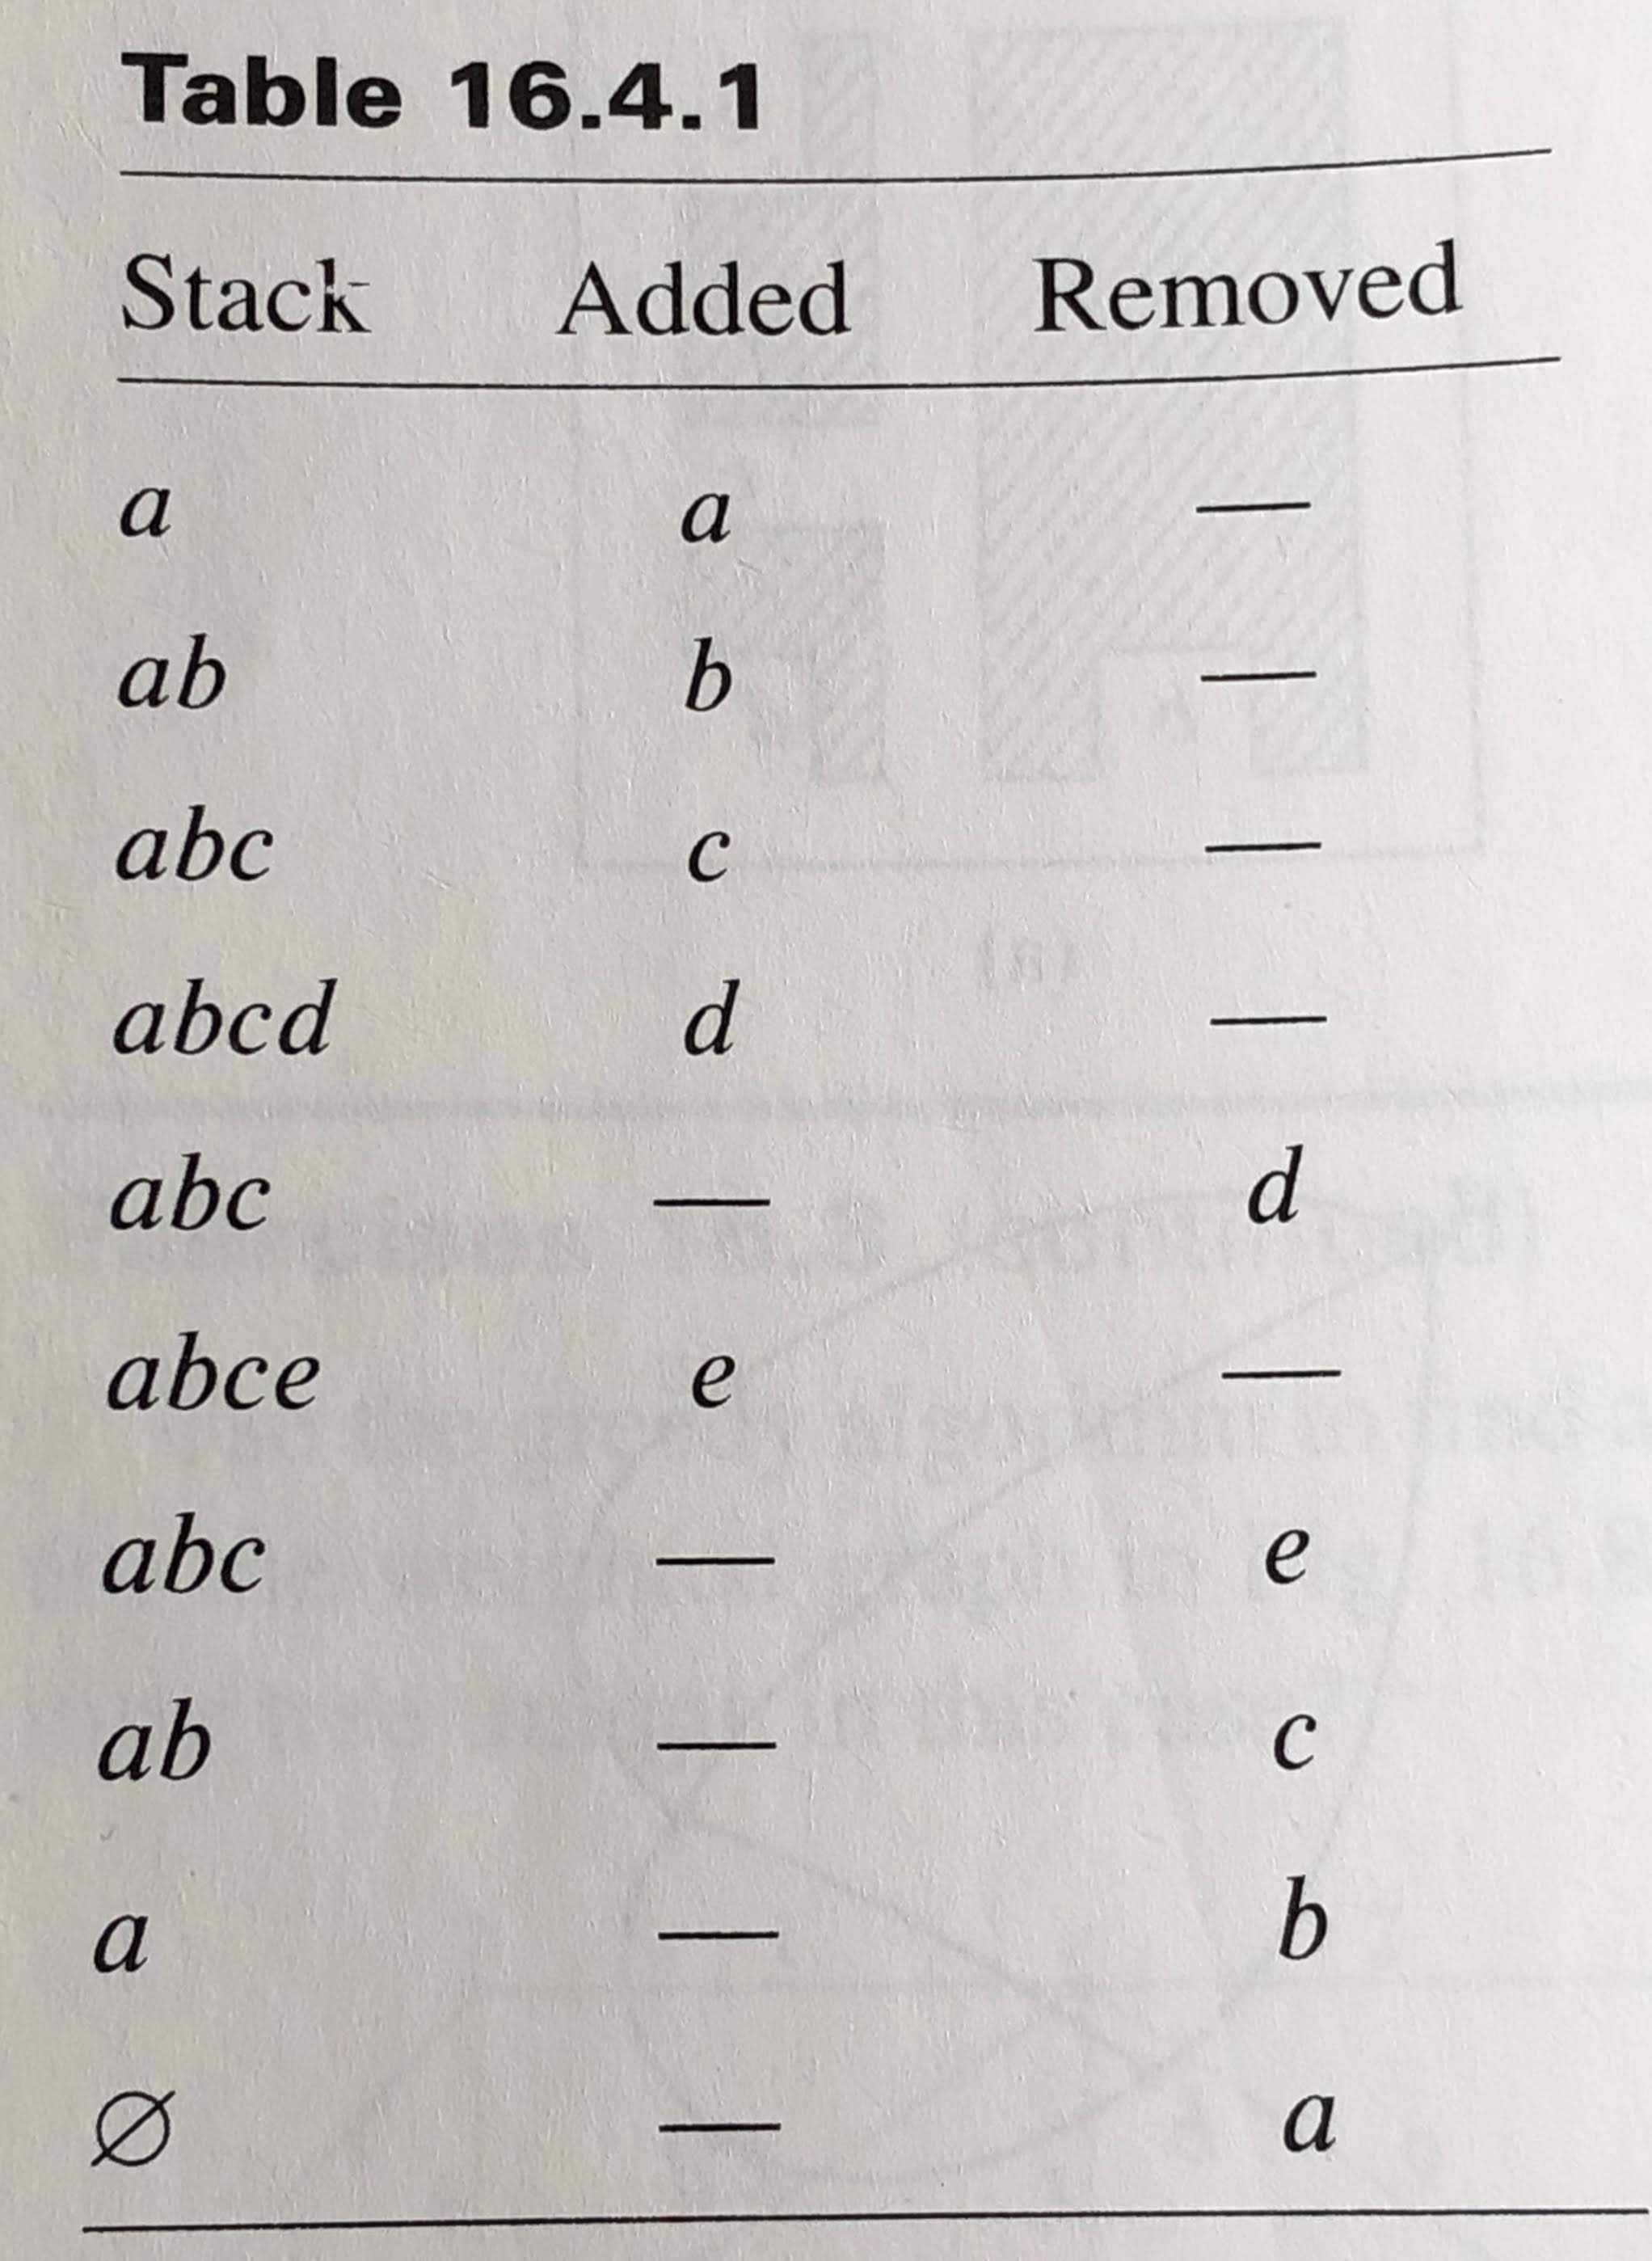
\includegraphics[width=0.17\textwidth]{images/DFS_dia}


\subsection{Breadth-first search (BFS)}
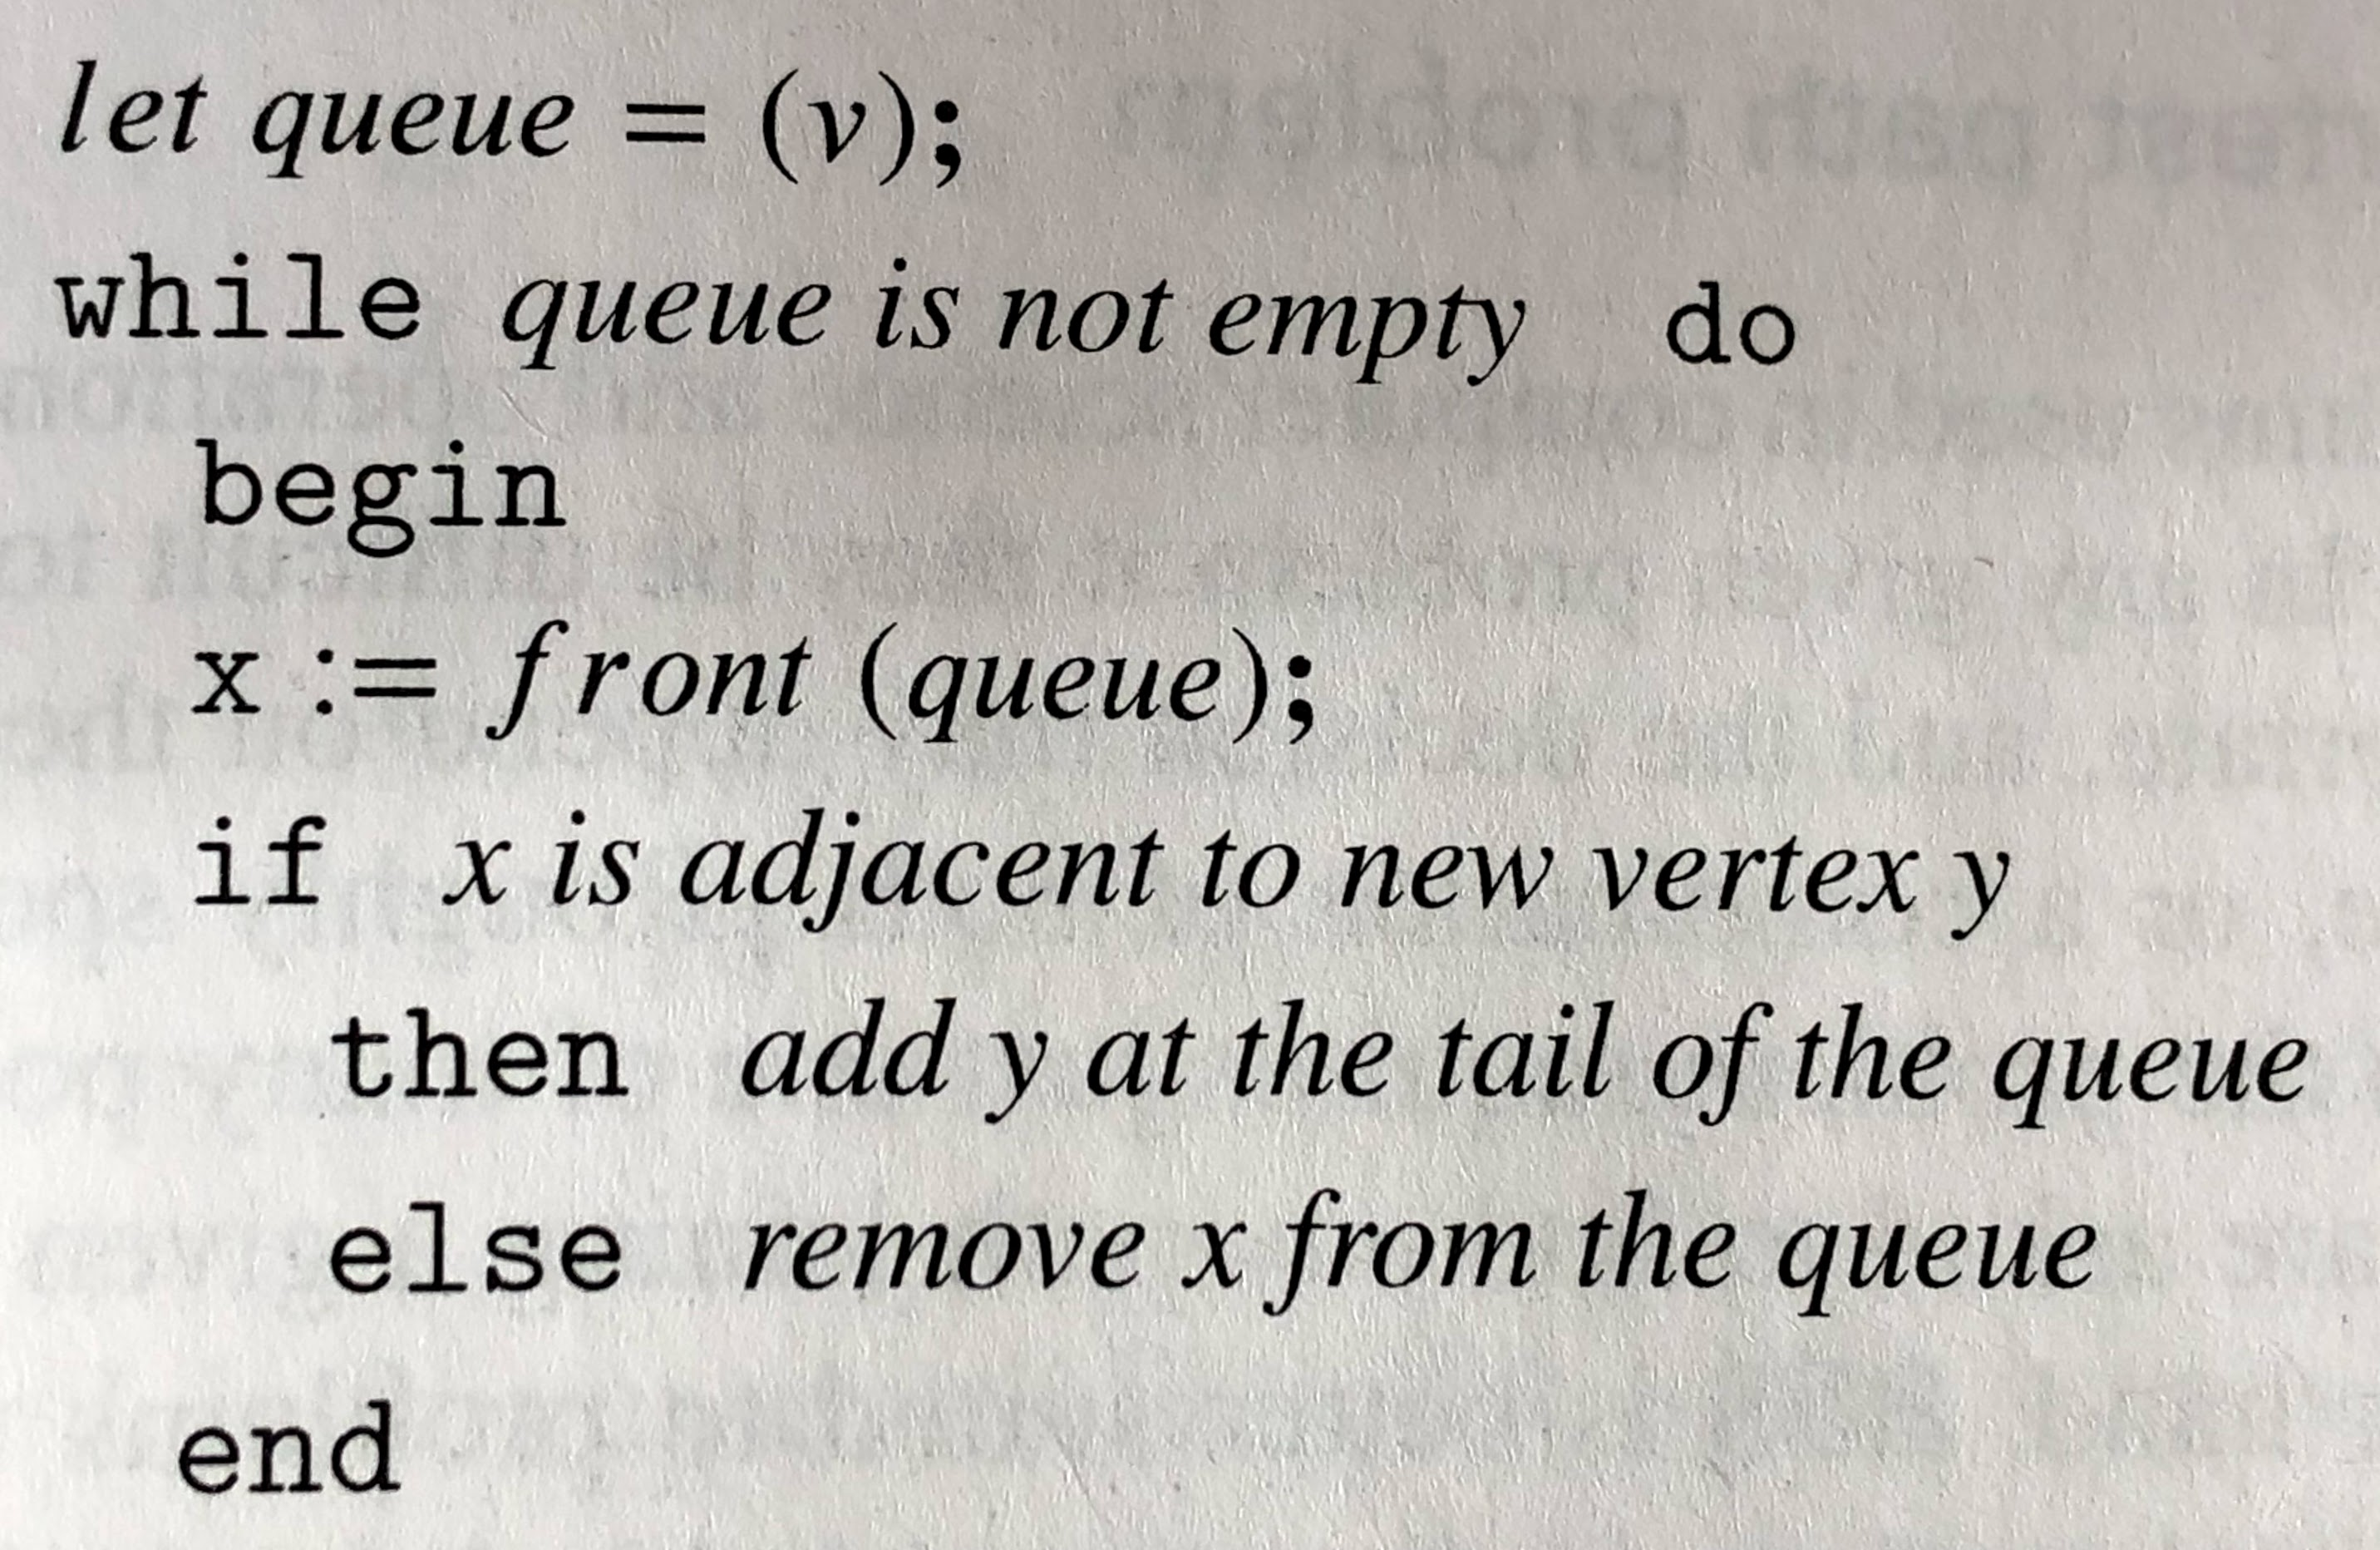
\includegraphics[width=0.25\textwidth]{images/BFS_alg}
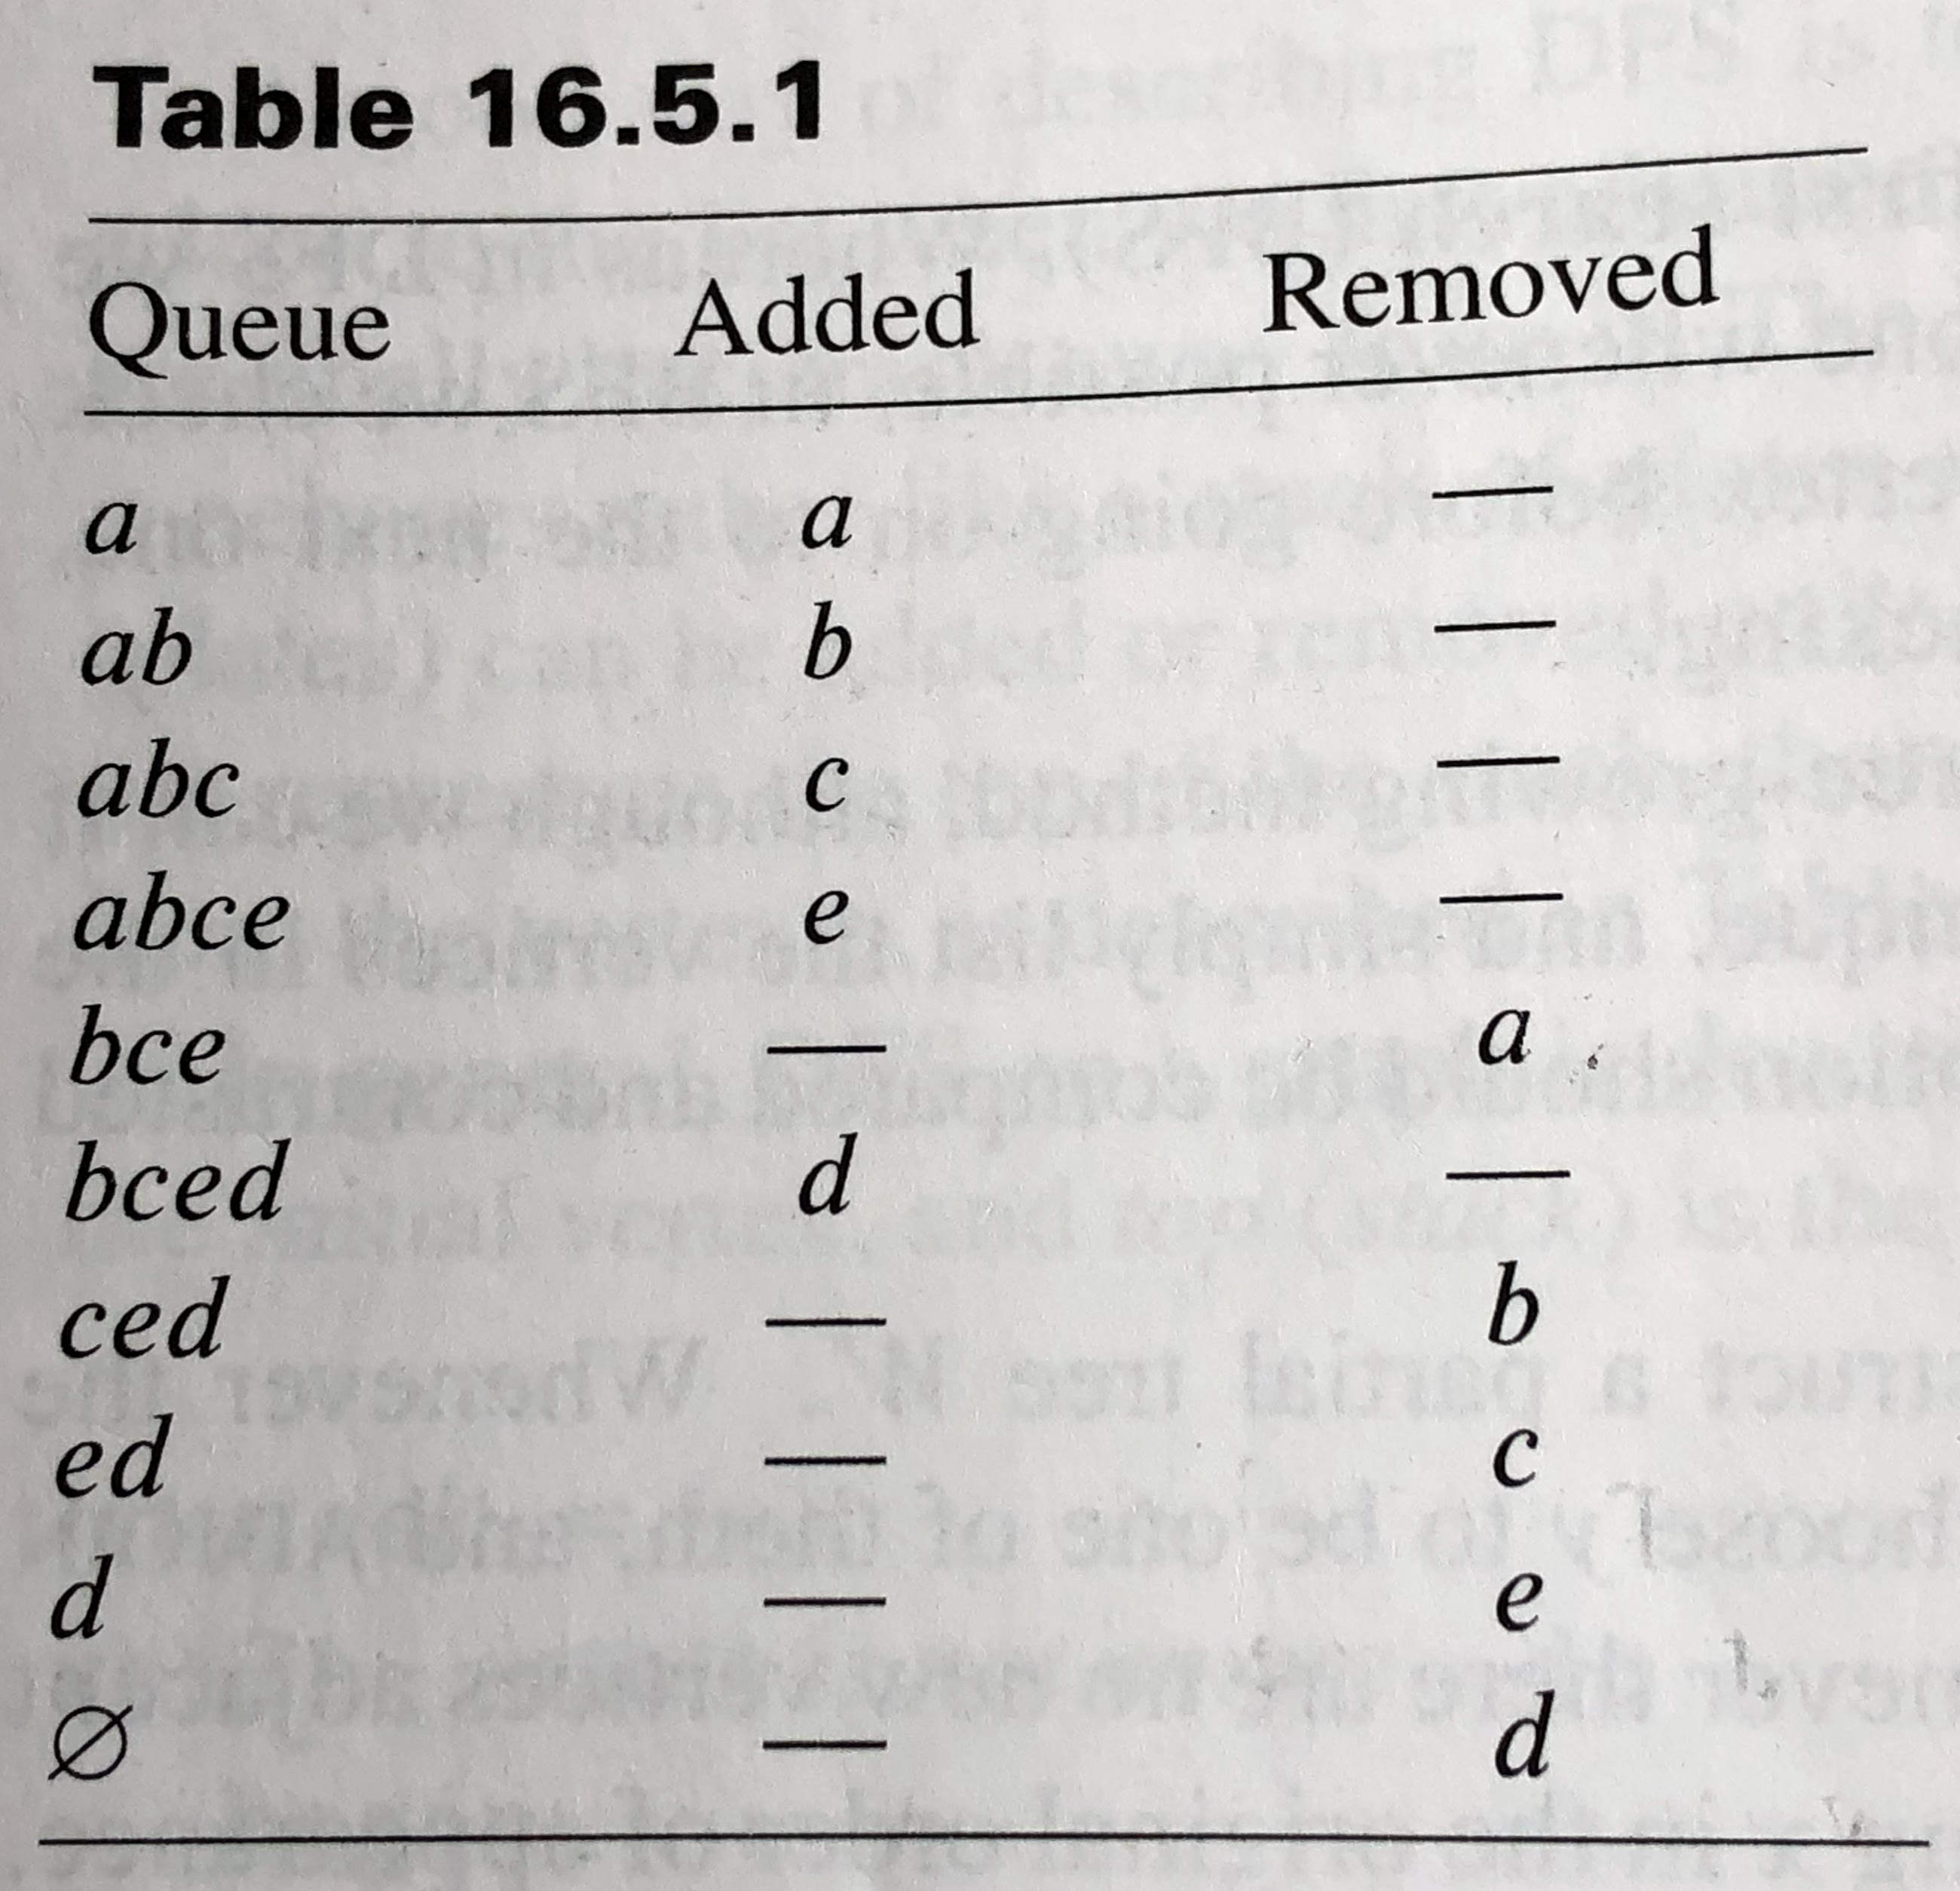
\includegraphics[width=0.2\textwidth]{images/BFS_dia}

\subsection{Shortest path problem (Dijkstras algoritm)}
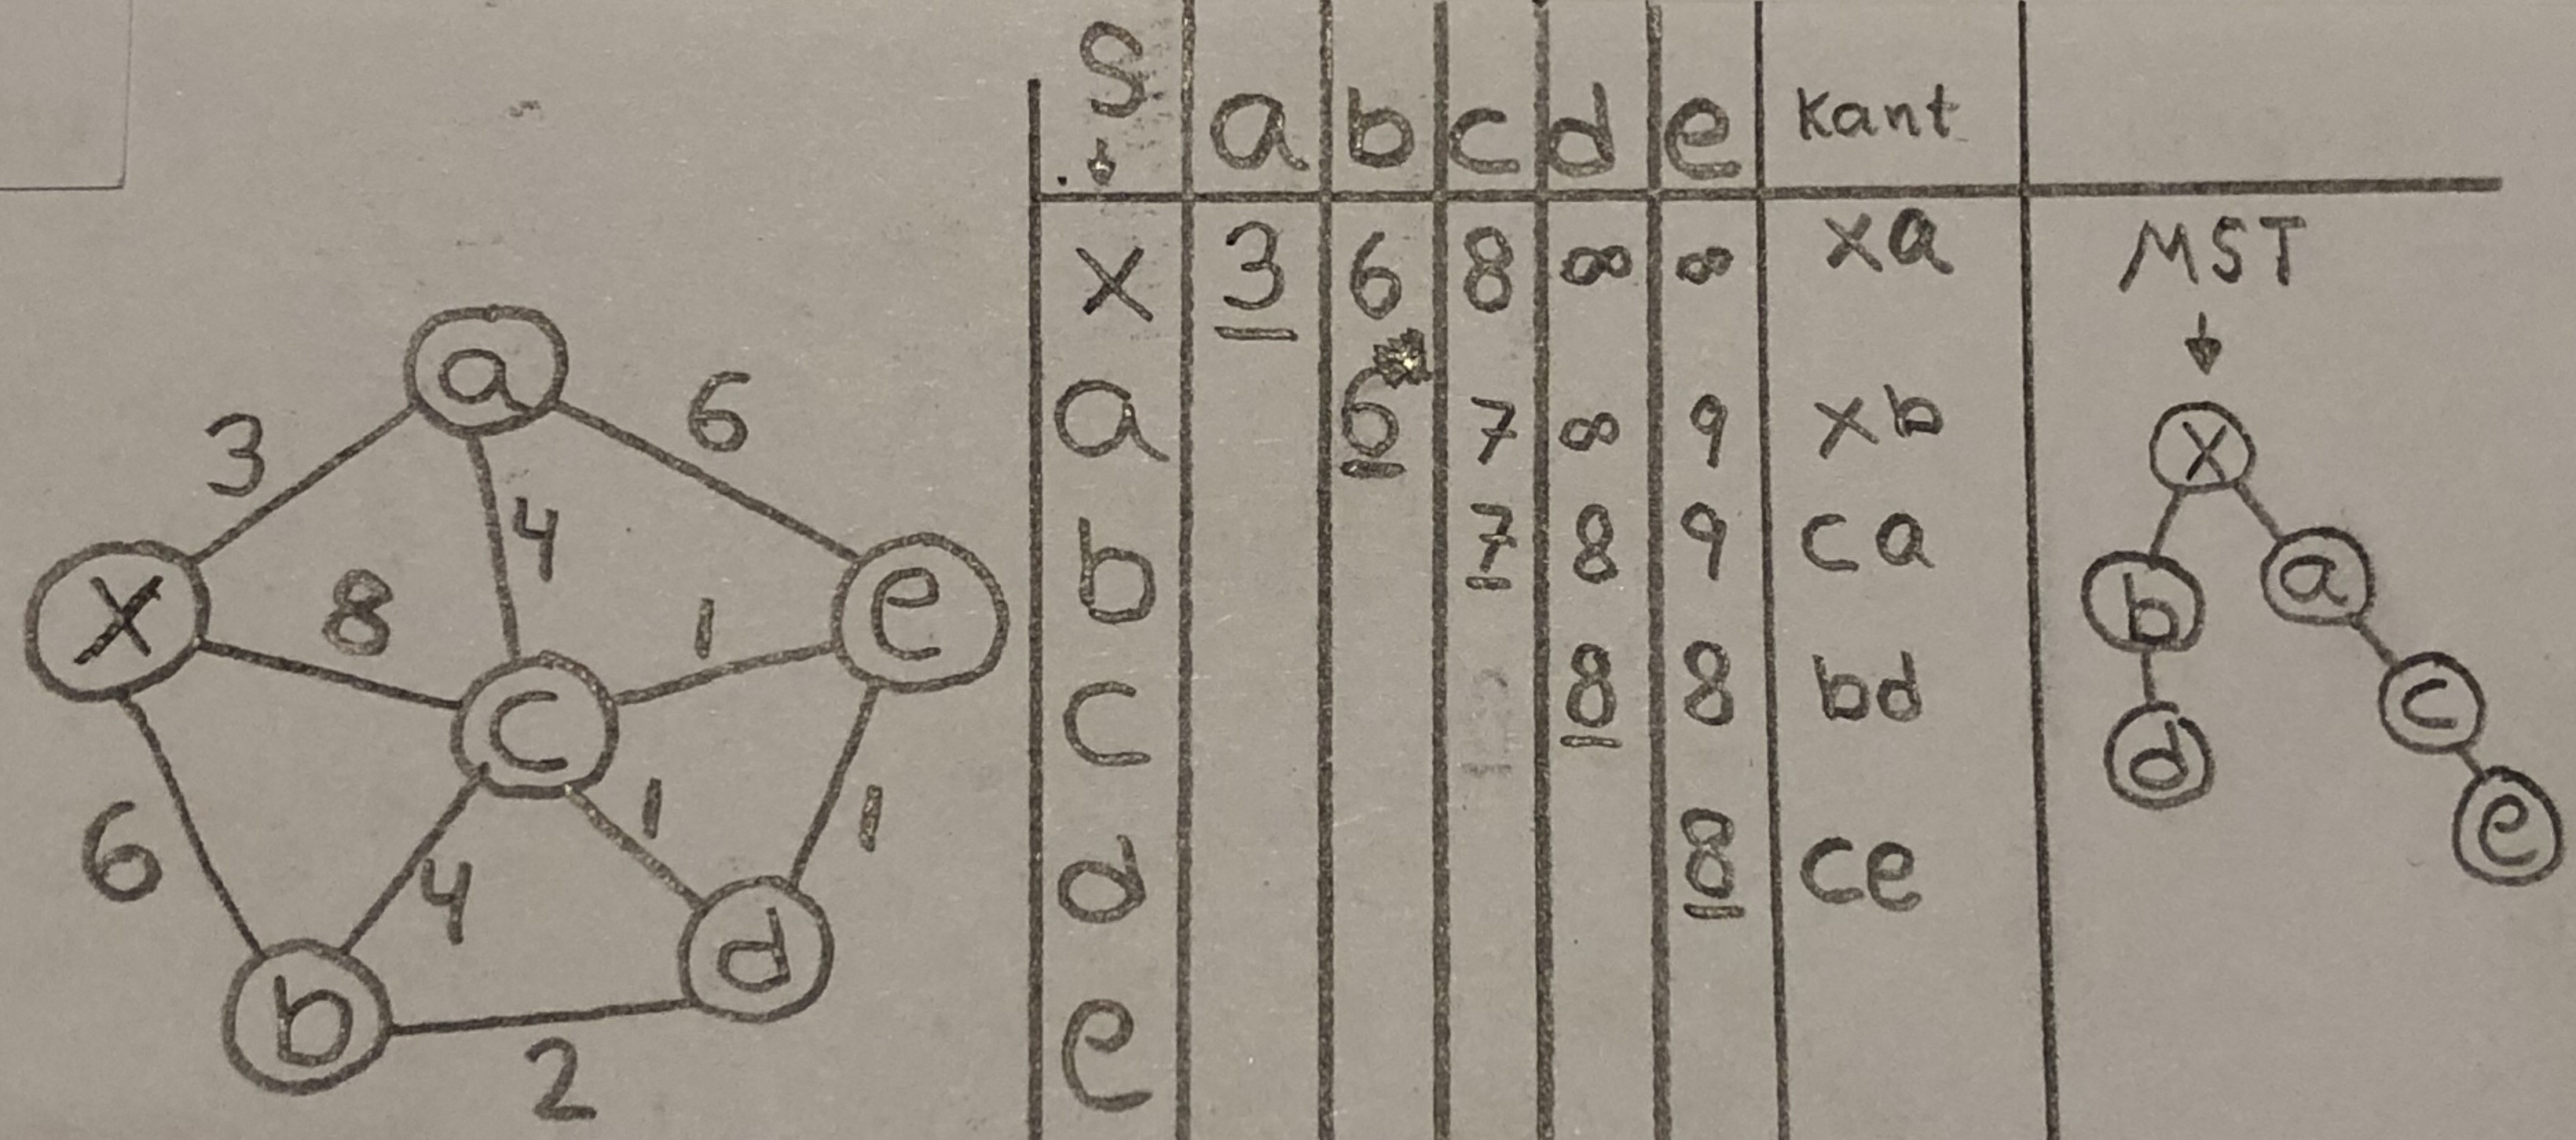
\includegraphics[width=0.48\textwidth]{images/kortast}
Förklaring: $S$ är mängden av alla besökta kanter. (*) 6:an i bilden (ab) ges av $min(L(b),L(a)+w(ab))=min(6,3+\infty)=6$, där $L(b)$ är den tidigare vägen till $b$ och $w(ab)$ är vikten på kanten $ab$ vilket inte existerar och därmed är $\infty$. Till höger i bild är det minimalt uppspännande trädet som erhålls från kant-kolumnen. \textbf{På en tenta} blir våra kära matematiker mycket glada om du bifogar det minimalt uppspännande trädet.
    \subsection{Bipartite \& Matchings}
    
    
    \textbf{Theorem 15.7.2}\\
    A graph is \textbf{bipartite} if and only if it contains no cycles with odd length. Alternativt: Om $\chi(G) = 2$, minsta antal färgningar är 2.\\
    \newline
    \textbf{Definition:} A \textbf{matching} in a bipartite graph $G = (U \cup Y, E)$ is a subset $M$ of $E$ with the property that no two edges in $M$ have a common vertex. Mängd av kanter som inte har hörn gemensamt (parvis).\\
    \newline
    \textbf{Definition:} We shall say that a matching $M$ is a \textbf{maximum matching} for $G = (U \cup Y, E)$ if no other matching has a greater cardinality.\\
    \newline
    \textbf{Definition:} If $|M|=|X|$ then we say that $M$ is a \textbf{complete matching} (\textbf{komplett/perfekt matchning}). \\
    \newline
    \textbf{Theorem 17.4}\\
    The bipartite graph $G = (U \cup Y, E)$ has a complete matching if and only if Hall's condition is satisfied, that is 
    $$|J(A)| \geq |A| \quad \text{for all} \quad A \subseteq X.$$ 
\end{multicols}
\end{document}
